    \chapter{Modelação do Domínio Comum}

    \section{Visão Global do Domínio}

    No final do estudo prévio realizado no capítulo anterior, verificou-se uma acentuada fragmentação estrutural entre os principais fornecedores de Modelos de Linguagem de Grande Escala (LLMs) [13]. A ausência de uma padronização ou um protocolo comum leva à inconsistencia entre as APIs da OpenAI [1], Anthropic [2] e Gemini [3] , as quais têm campos distintos, diferentes ciclos de vida para o fluxo de dados e estruturas de objetos incompatíveis entre as várias APIs.

    Para garantir a interoperabilidade, a arquitetura do OmniAI SDK assenta na criação de um modelo de domínio comum. A ideia foi criar um modelo de dados intereoperavel com os maiores forncessedores de inferencia para representar pedidos, respostas e eventos dos mesmos, mas sem copiar diretamente a estrutura de nenhum deles.

   Assim, o domínio funciona como um ponto intermédio estável que centraliza qualquer interação no OmniAI SDK. Isto significa que, independentemente de o cliente estruturar o seu pedido original no formato de um fornecedor específico (como por exemplo a Anthropic), esse contrato é imediatamente convertido para o domínio unificado e em seguida, para efetuar a chamada à API, o modelo comum é novamente traduzido para o formato nativo do fornecedor de destino. O mesmo processo inverso ocorre na receção da resposta, os dados que são devolvidos pela API externa são normalizados no nosso domínio comum antes de serem entregues ao cliente na estrutura esperada. Este fluxo completo de transformações está representado visualmente na Figura 3.1.
   
   
\begin{figure}[H]
    \centering
    \begin{tikzpicture}[
        node distance=0.8cm and 0.5cm,
        % font=\small e larguras ajustadas garantem que o texto não transborda
        box/.style={rectangle, draw, rounded corners, align=center, text width=3.5cm, minimum height=1.2cm, inner sep=4pt, thick, font=\small},
        common/.style={rectangle, draw, rounded corners, align=center, text width=3.2cm, minimum height=1.2cm, inner sep=4pt, fill=gray!20, thick, font=\small},
        api/.style={rectangle, draw, rounded corners, align=center, text width=2.4cm, minimum height=1.2cm, inner sep=4pt, fill=blue!5, dashed, thick, font=\small},
        arrow/.style={-Latex, thick}
    ]
        % --- LINHA DE PEDIDO (Cima) ---
        \node[box] (inReq) {Pedido recebido\\(OpenAI, Anthropic\\ou Gemini)};
        \node[common, right=of inReq] (commonReq) {\textbf{CommonRequest}};
        \node[box, right=of commonReq] (contractReq) {Contrato da API\\(OpenAI, Anthropic\\ou Gemini)};
        \node[api, right=of contractReq] (apiCall) {Chamada à API\\de Inferência};

        % --- LINHA DE RESPOSTA (Baixo) ---
        \node[api, below=1.2cm of apiCall] (apiResp) {Resposta da API\\de Inferência};
        \node[box, left=of apiResp] (contractResp) {Contrato da API\\(OpenAI, Anthropic\\ou Gemini)};
        \node[common, left=of contractResp] (commonResp) {\textbf{CommonResponse}\\ou \textbf{...Event}};
        \node[box, left=of commonResp] (clientResp) {Resposta Cliente\\(OpenAI, Anthropic\\ou Gemini)};

        % --- LIGAÇÕES ---
        % Fluxo de Ida
        \draw[arrow] (inReq) -- (commonReq);
        \draw[arrow] (commonReq) -- (contractReq);
        \draw[arrow] (contractReq) -- (apiCall);
        
        % Transição Lógica (Processamento pela API)
        \draw[arrow, dashed] (apiCall) -- (apiResp);

        % Fluxo de Volta
        \draw[arrow] (apiResp) -- (contractResp);
        \draw[arrow] (contractResp) -- (commonResp);
        \draw[arrow] (commonResp) -- (clientResp);
    \end{tikzpicture}
    \caption{Fluxo de normalização entre contratos externos e domínio comum (OmniAi-SDK)}
    \label{fig:domain-overview}
\end{figure}

    \section{{Estrutura do Domínio Comum}}
    O domínio comum do \textbf{OmniAI SDK} que consite no conjunto de classes e relações que padroniza as interações com os diferentes fornecedores divide-se em dois blocos principais: \textbf{Request} e \textbf{Response}.

    \begin{itemize}
        \item O \textbf{Request} define a estrutura dos pedidos enviados ao modelo.
        \item O \textbf{Response} descreve as respostas devolvidas, quer no formato (\texttt{CommonResponse}), quer em formato incremental atraves de eventos (\texttt{CommonResponseEvent}).
    \end{itemize}

    \subsection{{Request}}

    O \texttt{CommonRequest} é o modelo base que normaliza qualquer pedido a LLMs, garantindo um contrato único e consistente, independentemente do fornecedor. A estrutura foi desenhada para manter os elementos essenciais de geração (fornecedor, modelo e mensagens) e, ao mesmo tempo, permitir extensões controladas via configuração e opções específicas do provider.
    Como se observa na Figura 3.2, o \texttt{CommonRequest} agrega diretamente o \texttt{provider}, o \texttt{model} e a lista de \texttt{messages}, que representam o histórico conversacional. Cada \texttt{CommonRequestMessage} contém o papel (\texttt{CommonRole}) e o conteúdo em partes (\texttt{RequestContentPart}), permitindo combinar texto, JSON ou chamadas a ferramentas. A configuração de geração é isolada em \texttt{CommonGenerationConfig}, enquanto as ferramentas disponíveis são descritas por \texttt{CommonTool} e controladas por \texttt{ToolChoice}. Por fim, \texttt{SystemPrompt} e \texttt{providerOptions} suportam personalizações globais e específicas do fornecedor, mantendo o núcleo estável e extensível.


    \begin{figure}[H]
        \centering
        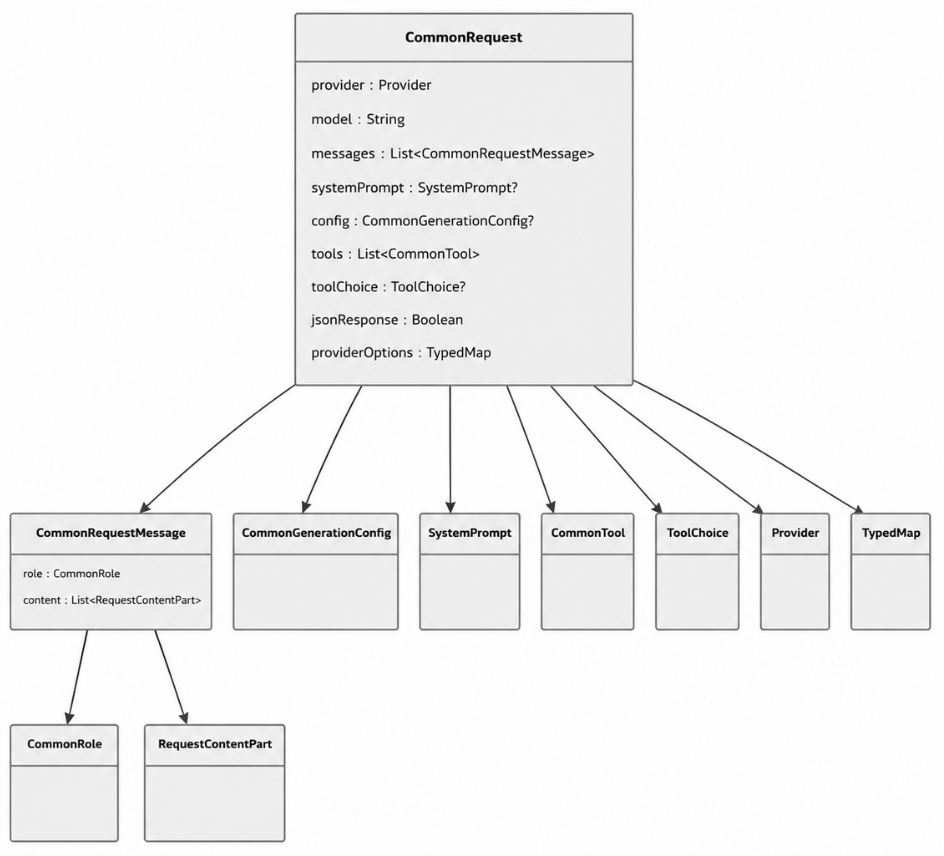
\includegraphics[width=0.95\textwidth]{../images/CommonRequestClasses}
        \caption{Estrutura de classes do \texttt{CommonRequest}.}
        \label{fig:commonrequest-classes}
    \end{figure}

    Para sistematizar a estrutura apresentada na Figura 3.2, a Tabela~\ref{tab:request-parametros} agrega todos os parâmetros relevantes do domínio de \textit{Request}, incluindo o objeto principal e os tipos diretamente associados. O objetivo é apresentar o significado funcional de cada campo no fluxo de construção do pedido.

    \begin{table}[H]
    \centering
    \footnotesize
    \setlength{\tabcolsep}{4pt}
    \renewcommand{\arraystretch}{1.15}
    \begin{tabularx}{\textwidth}{|>{\raggedright\arraybackslash}p{2.6cm}|>{\raggedright\arraybackslash}p{3.0cm}|>{\raggedright\arraybackslash}p{2.9cm}|>{\raggedright\arraybackslash}X|}
    \hline
    \textbf{Elemento} & \textbf{Campo} & \textbf{Tipo} & \textbf{Descrição} \\ \hline

    CommonRequest & provider & Provider & Fornecedor alvo da chamada. \\ \hline
    CommonRequest & model & String & Identificador do modelo a utilizar. \\ \hline
    CommonRequest & messages & \texttt{List\textless\allowbreak Common\allowbreak Request\allowbreak Message\textgreater} & Histórico de mensagens enviado ao modelo. \\ \hline
    CommonRequest & systemPrompt & SystemPrompt? & Prompt de sistema global (opcional). \\ \hline
    CommonRequest & config & CommonGenerationConfig? & Parâmetros de geração (opcional). \\ \hline
    CommonRequest & tools & \texttt{List\textless\allowbreak Common\allowbreak Tool\textgreater} & Ferramentas disponíveis para chamadas de função. \\ \hline
    CommonRequest & toolChoice & ToolChoice? & Política de seleção de ferramentas. \\ \hline
    CommonRequest & jsonResponse & Boolean & Indica se a resposta deve ser forçada a JSON. \\ \hline
    CommonRequest & providerOptions & TypedMap & Opções específicas do fornecedor. \\ \hline

    \texttt{Common\allowbreak Request\allowbreak Message} & role & CommonRole & Papel da mensagem (SYSTEM, USER, ASSISTANT, TOOL). \\ \hline
    \texttt{Common\allowbreak Request\allowbreak Message} & content & \texttt{List\textless\allowbreak Request\allowbreak Content\allowbreak Part\textgreater} & Conteúdo segmentado da mensagem. \\ \hline

    SystemPrompt & text & String & Conteúdo do prompt de sistema. \\ \hline

    \texttt{Common\allowbreak Generation\allowbreak Config} & temperature & Double? & Grau de aleatoriedade da geração. \\ \hline
    \texttt{Common\allowbreak Generation\allowbreak Config} & maxTokens & Int? & Limite máximo de tokens de saída. \\ \hline
    \texttt{Common\allowbreak Generation\allowbreak Config} & topP & Double? & Probabilidade cumulativa (nucleus sampling). \\ \hline
    \texttt{Common\allowbreak Generation\allowbreak Config} & stopSequences & \texttt{List\textless\allowbreak String\textgreater}? & Sequências que interrompem a geração. \\ \hline

    CommonTool & name & String & Nome da ferramenta. \\ \hline
    CommonTool & description & String & Descrição funcional da ferramenta. \\ \hline
    CommonTool & parametersSchema & JsonObjectMap & Esquema JSON dos parâmetros. \\ \hline

    ToolChoice & Auto/None/Required/Specific & -- & Estratégia de uso de ferramentas (auto, nenhuma, obrigatório ou lista específica). \\ \hline

    \texttt{Request\allowbreak Content\allowbreak Part} & TextPart & \texttt{text: String} & Conteúdo textual. \\ \hline
    \texttt{Request\allowbreak Content\allowbreak Part} & JsonPart & \texttt{json: JsonValue} & Conteúdo JSON estruturado. \\ \hline
    \texttt{Request\allowbreak Content\allowbreak Part} & ToolCallPart & \texttt{toolCallId, functionName, argumentsJson} & Chamada a ferramenta com argumentos. \\ \hline
    \texttt{Request\allowbreak Content\allowbreak Part} & ToolResultPart & \texttt{toolCallId, content} & Resultado de execução de ferramenta. \\ \hline

    \end{tabularx}
    \caption{Parâmetros do domínio de \textit{Request}.}
    \label{tab:request-parametros}
    \end{table}



    \subsection{{CommonResponse e CommonResponseEvent}}
